\setcounter{equation}{0}
\chapter{Results and Discussion}
\label{chap:results}

This chapter presents the outcomes of Phase 1 of the project. The phase covered the digitization of the SJCET register, the construction of the regional dataset, the three-stage training of the forecasting model, its evaluation against conventional baselines, and the web application that presents the forecasts. All scores are computed at the SJCET node over the 2015--2016 test period, on every day for which the register has a reading.

\section{Dataset Preparation and Preprocessing Results}
\label{sec:res-data}

The digitization of the July 2010 -- December 2016 register produced a daily dataset of \textbf{1,549 observed days} out of 2,376 calendar days, with weekends and holidays accounting for most of the gaps (Figure~\ref{fig:coverage}). Every value is traceable to its page, and \textbf{59 of the 78 months} agree with the observers' own written rainfall totals to within 0.1\,cm. For six of the mismatched months a zoomed re-read showed the transcription to be correct and the error to be the observer's addition. Overall, 1,095 days are flagged \textbf{ok} and 454 \textbf{suspect}, mostly because of a monthly rain-total mismatch that casts doubt on the rain values rather than the temperatures.

The register is unusual as a training target. It is read only on weekdays, it records most temperatures in whole degrees, its rain gauge is emptied only when read, and its maximum thermometer often shows the same value for weeks. After the 08:30 reading convention is applied and accumulated or doubtful values are removed, the training period contains \textbf{716 temperature days} and only \textbf{249 rain days}.

The regional dataset joins 36 years (1990--2025) of NASA POWER reanalysis at 1,062 grid points, six NOAA stations and the SJCET node into a single graph of \textbf{1,069 nodes and 8,884 edges} (Figure~\ref{fig:graphmap}). It provides 8,754 training days for stages 1 and 2, against 1,194 candidate days for stage 3 at SJCET.

\begin{figure}[!htbp]
    \centering
    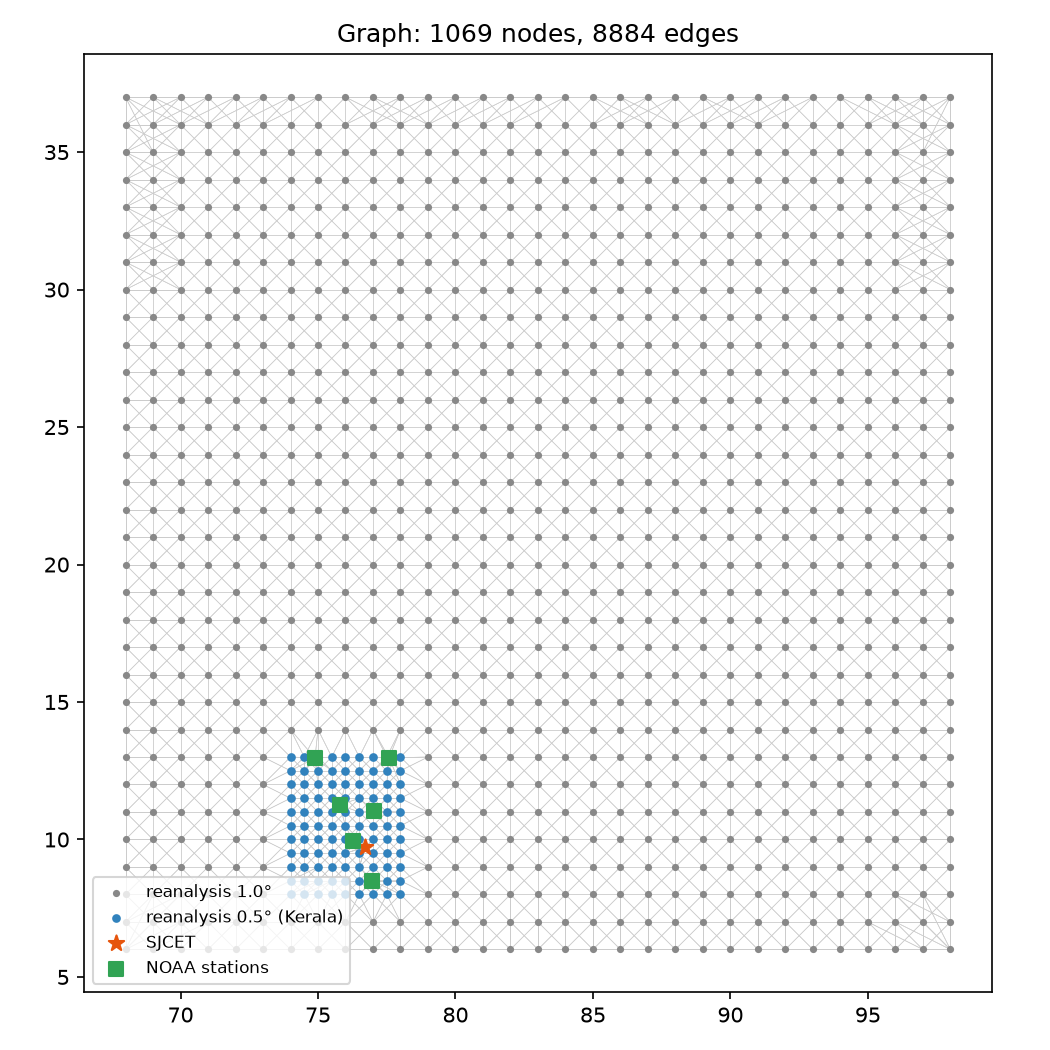
\includegraphics[width=0.62\textwidth]{graph_map.png}
    \caption{\capFigGraphMap}\label{fig:graphmap}
\end{figure}

\section{Training Progress}
\label{sec:res-training}

The model was trained in three stages on a CPU. Stage 1, first trained at a one-day horizon, was continued for 4 epochs at the six-day horizon; its validation loss fell from 0.357 to 0.344, at about 400 seconds per epoch over the full 1,069-node graph. Stage 2 ran for a further 4 epochs and its validation loss fell from 0.385 to 0.379. Stage 3 trains on SJCET's 4-hop subgraph only, so each epoch takes about 12 seconds. The pretrained models reached their lowest validation loss after 2 epochs (0.722 for 1$\to$\allowbreak{}2$\to$\allowbreak{}3) and early stopping ended training after 6, while the network trained from scratch needed 5 epochs and fluctuated much more between epochs. A pretrained network therefore needs very little local training to adapt.

The results are reproducible. For this report the evaluation was re-run on a separate machine (\textbf{train.py -{}-eval-only}) and reproduced every score to two decimal places, and the main stage-3 model was retrained from the stage-2 checkpoint (\textbf{train.py -{}-stage 3 -{}-init s12/\allowbreak{}best.pt -{}-fraction 1.0 -{}-seed 0}) and matched the original training log at every epoch.

\section{Forecast Accuracy}
\label{sec:res-accuracy}

Forecast accuracy is the headline result of the project. For temperature it is measured as $100-\mathrm{MAPE}$, the percentage by which a forecast agrees with the register reading, and for rain as the percentage of days on which the forecast correctly says whether it rains ($\geq$2.5\,mm). Table~\ref{tab:accuracy} gives both for every model, one and six days ahead, and Figure~\ref{fig:timeseries} compares the next-day forecasts of the final model with the register over the whole test period.

\begin{table}[!htbp]
    \centering
    \caption{\capTabAccuracy}\label{tab:accuracy}
    \footnotesize
    \begin{tabularx}{\textwidth}{|L{4.6cm}|C{1.45cm}|C{1.45cm}|C{1.45cm}|C{1.45cm}|Y|}
        \hline
        \textbf{Model} & \textbf{Tmax d1 (\%)} & \textbf{Tmin d1 (\%)} & \textbf{Tmax d6 (\%)} & \textbf{Tmin d6 (\%)} & \textbf{Rain/no-rain d1 (\%)} \\ \hline
        GNN 1$\to$\allowbreak{}2$\to$\allowbreak{}3 (region$\to$\allowbreak{}stations$\to$\allowbreak{}SJCET) & 96.6 & 96.2 & 96.3 & 95.8 & 64.0 \\ \hline
        GNN 1$\to$\allowbreak{}3 (region$\to$\allowbreak{}SJCET) & 96.7 & 96.1 & \textbf{96.4} & 95.6 & 63.3 \\ \hline
        GNN from scratch (SJCET only) & 94.9 & 94.1 & 95.7 & 94.8 & 63.3 \\ \hline
        GNN stage 1 only (no SJCET data) & 91.0 & 91.3 & 89.9 & 92.0 & 73.8 \\ \hline
        GNN stages 1$\to$\allowbreak{}2 (no SJCET data) & 90.9 & 91.6 & 90.1 & 92.5 & 73.5 \\ \hline
        XGBoost (station + nearest grid) & 96.6 & 96.4 & 96.1 & 95.6 & 53.8 \\ \hline
        Climatology & 95.3 & 95.7 & 95.4 & 95.7 & 50.9 \\ \hline
        Persistence & \textbf{97.8} & \textbf{97.8} & \textbf{96.4} & \textbf{96.0} & 75.3 \\ \hline
        Reanalysis at nearest grid node & 87.8 & 94.7 & 87.8 & 94.7 & \textbf{77.5} \\ \hline
    \end{tabularx}
\end{table}

\begin{figure}[!htbp]
    \centering
    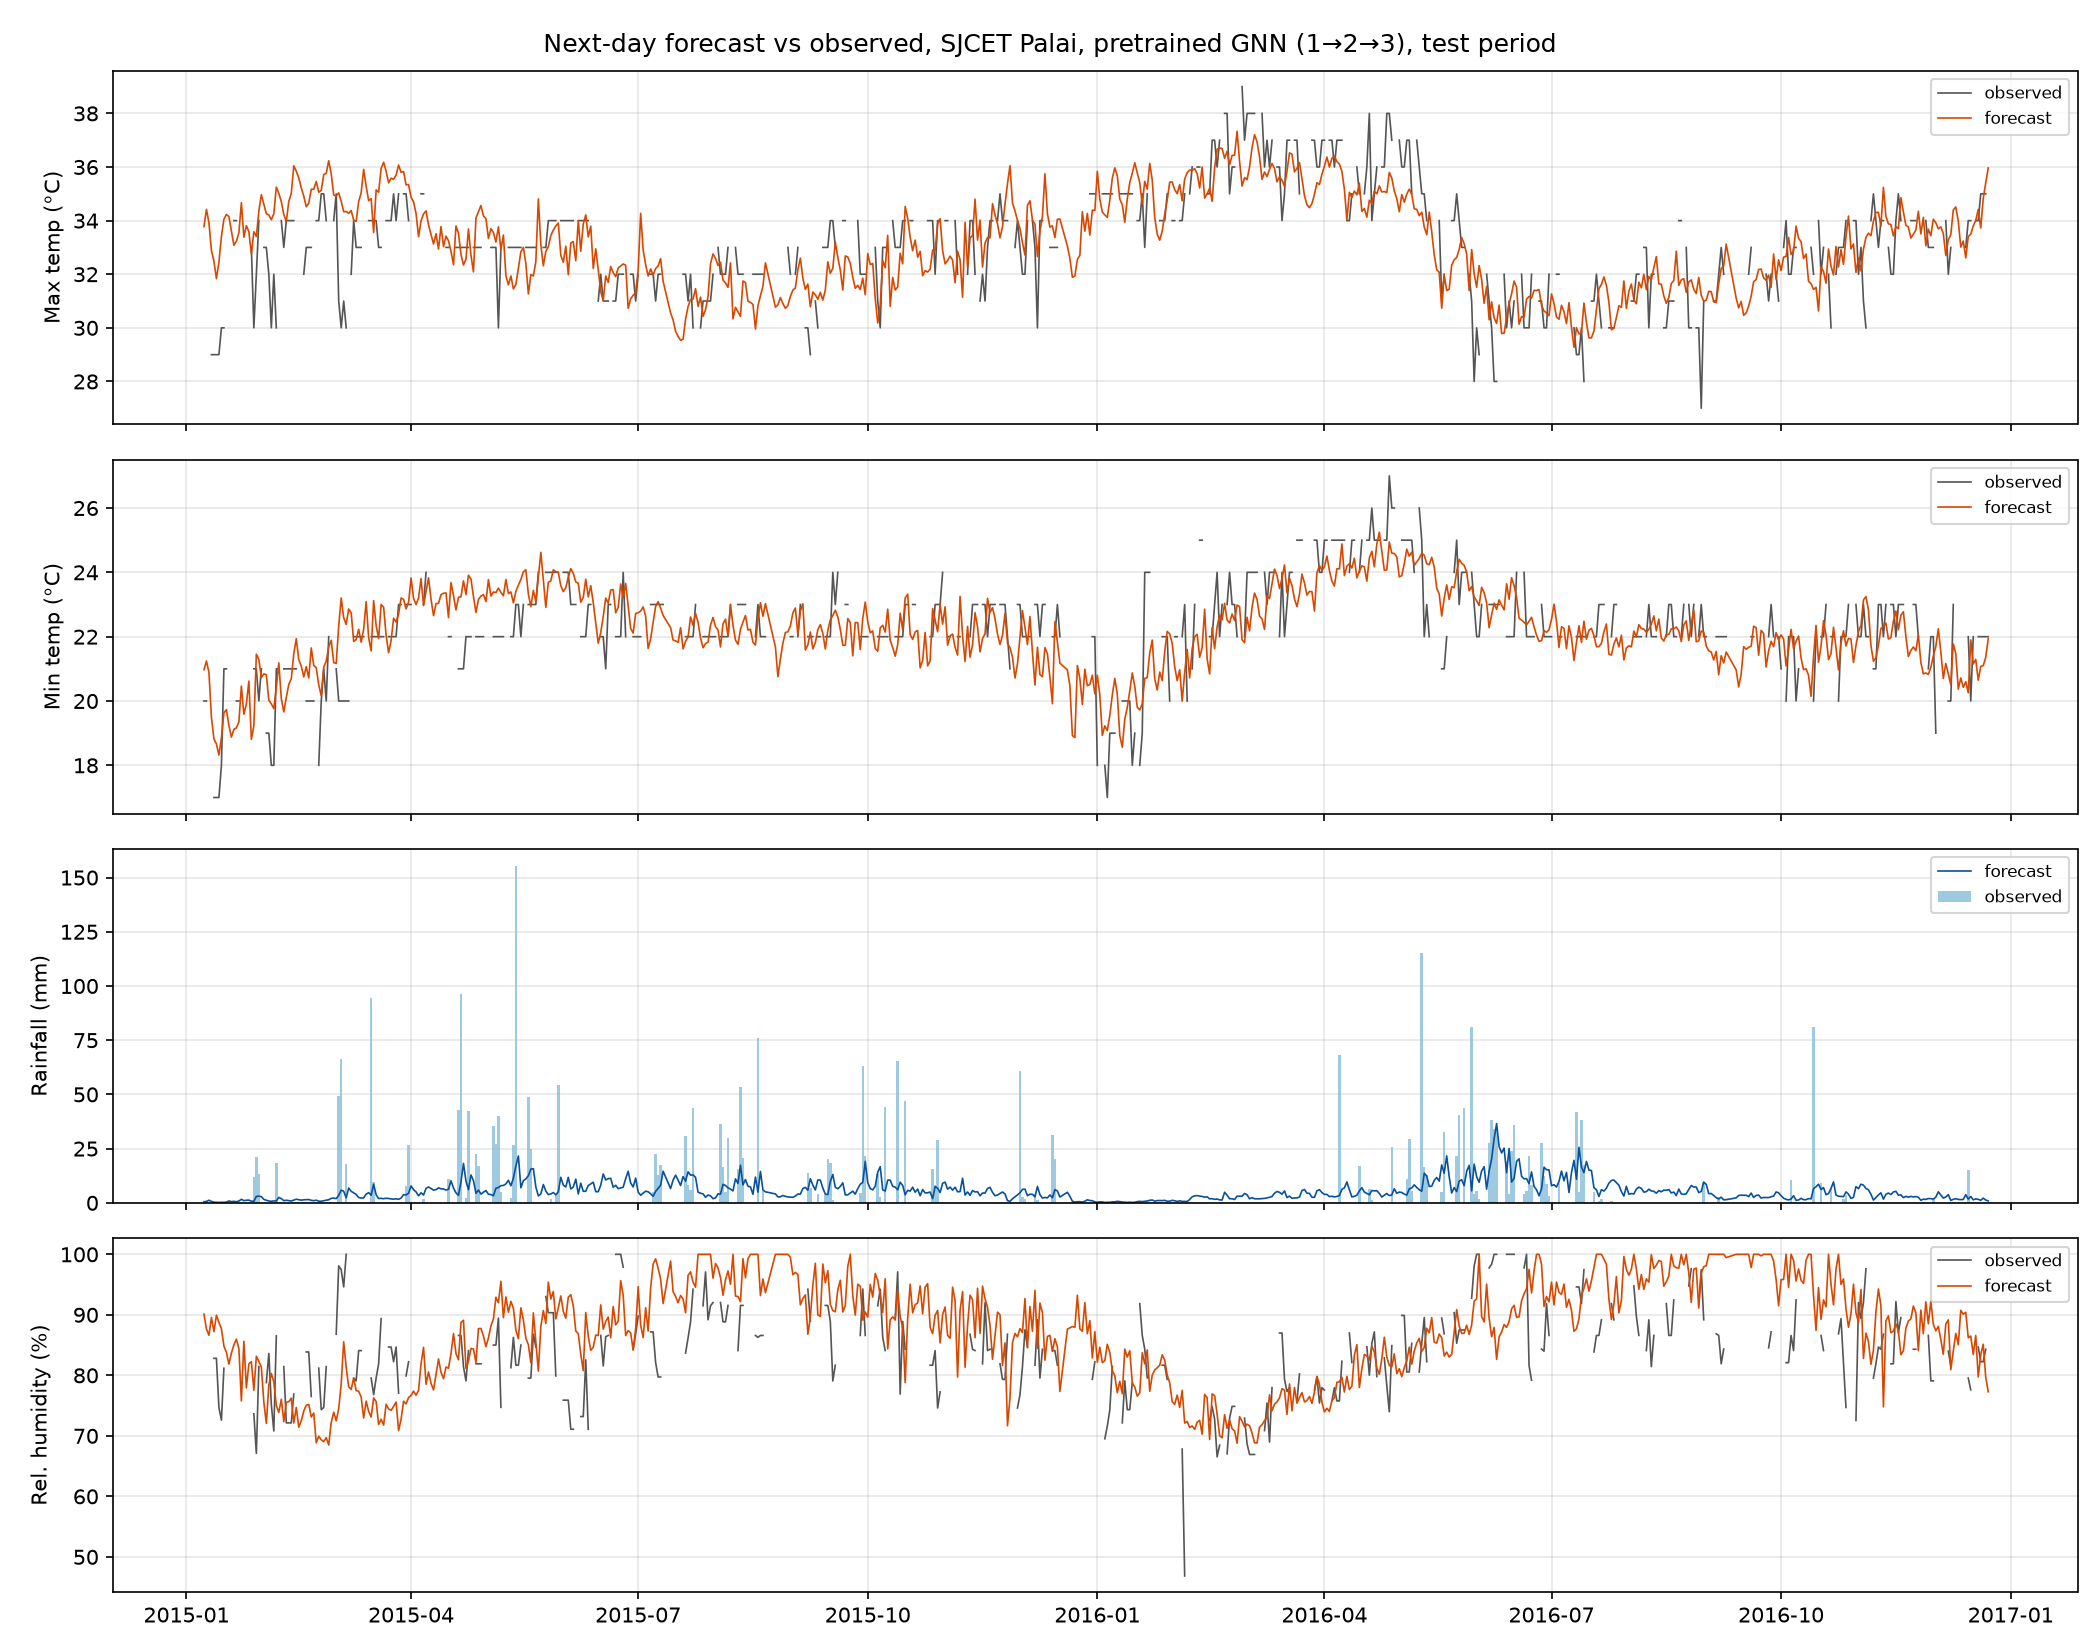
\includegraphics[width=0.95\textwidth]{test_timeseries.png}
    \caption{\capFigTimeseries}\label{fig:timeseries}
\end{figure}

\begin{itemize}
    \item \textbf{The final model forecasts temperature with about 96\% accuracy.} The region$\to$\allowbreak{}stations$\to$\allowbreak{}SJCET model forecasts the next day's maximum temperature with \textbf{96.6\%} accuracy and the minimum with \textbf{96.2\%}. In practical terms, \textbf{86\%} of its maximum-temperature forecasts and \textbf{93\%} of its minimum-temperature forecasts fall within $\pm$2\,\textdegree C of the register reading (55\% and 65\% within $\pm$1\,\textdegree C). Accuracy stays above 95.7\% six days ahead.
    \item \textbf{Pretraining is what delivers this accuracy.} The same network trained only on SJCET reaches 94.9\% and 94.1\%, with only 62\% of maximum-temperature forecasts within $\pm$2\,\textdegree C. Models that never see SJCET reach only about 91\%.
    \item \textbf{Against the baselines}, the pretrained GNNs are level with XGBoost and ahead of climatology. Persistence is the most accurate one day ahead (97.8\%), because the register repeats whole-degree values for days at a time, but by day 6 it falls to the level of the pretrained GNNs.
    \item \textbf{Rain is the weakest variable.} The fine-tuned GNNs call rain or no rain correctly on 63--64\% of days, below persistence (75\%) and the raw reanalysis (78\%).
\end{itemize}

\section{Error Comparison with Baselines}
\label{sec:res-full}

Table~\ref{tab:results} gives the same comparison as root-mean-square error (RMSE), and Figure~\ref{fig:rmse} shows it at every lead day.

\begin{table}[!htbp]
    \centering
    \caption{\capTabResults}\label{tab:results}
    \footnotesize
    \begin{tabularx}{\textwidth}{|L{3.9cm}|C{1.2cm}|C{1.2cm}|C{1.2cm}|C{1.45cm}|C{1.2cm}|Y|}
        \hline
        \textbf{Model} & \textbf{Tmax d1 (\textdegree C)} & \textbf{Tmin d1 (\textdegree C)} & \textbf{Rain d1 (mm)} & \textbf{Rain occ.\ acc.\ d1} & \textbf{Tmax d6 (\textdegree C)} & \textbf{Tmin d6 (\textdegree C)} \\ \hline
        GNN 1$\to$\allowbreak{}2$\to$\allowbreak{}3 (region$\to$\allowbreak{}stations$\to$\allowbreak{}SJCET) & 1.43 & 1.08 & 20.7 & 0.64 & 1.58 & \textbf{1.21} \\ \hline
        GNN 1$\to$\allowbreak{}3 (region$\to$\allowbreak{}SJCET) & 1.42 & 1.10 & 20.9 & 0.63 & \textbf{1.55} & 1.25 \\ \hline
        GNN from scratch (SJCET only) & 2.17 & 1.72 & 20.8 & 0.63 & 1.85 & 1.43 \\ \hline
        GNN stage 1 only (no SJCET data) & 3.40 & 2.16 & 22.6 & 0.74 & 3.75 & 2.04 \\ \hline
        GNN stages 1$\to$\allowbreak{}2 (no SJCET data) & 3.46 & 2.13 & 22.3 & 0.74 & 3.71 & 1.96 \\ \hline
        XGBoost (station + nearest grid) & 1.48 & 1.04 & 21.4 & 0.54 & 1.67 & 1.26 \\ \hline
        Climatology & 1.92 & 1.24 & 21.4 & 0.51 & 1.89 & 1.23 \\ \hline
        Persistence & \textbf{1.12} & \textbf{0.90} & 30.1 & 0.75 & 1.71 & 1.33 \\ \hline
        Reanalysis at nearest grid node & 4.55 & 1.58 & \textbf{20.5} & \textbf{0.78} & 4.56 & 1.59 \\ \hline
    \end{tabularx}
\end{table}

\begin{figure}[!htbp]
    \centering
    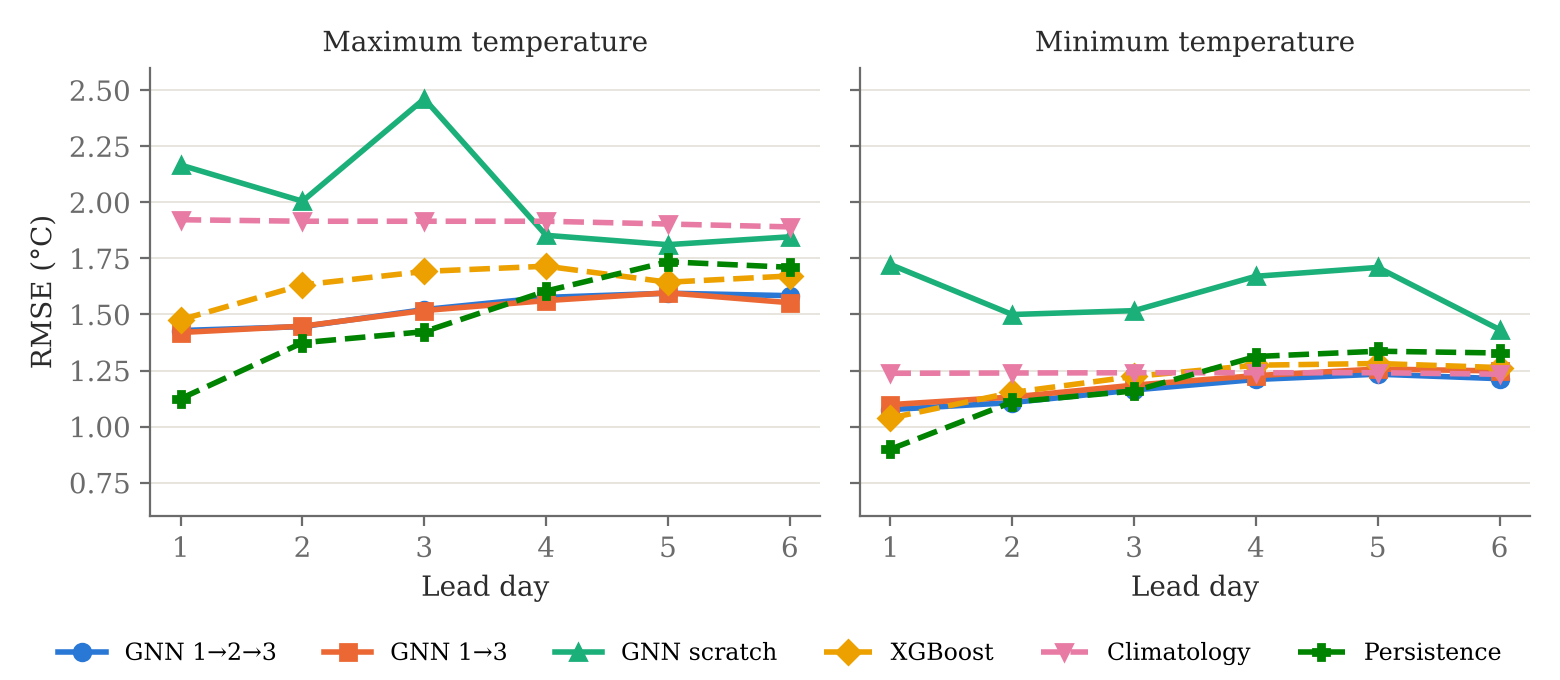
\includegraphics[width=0.98\textwidth]{rmse_lead.png}
    \caption{\capFigRmse}\label{fig:rmse}
\end{figure}

\begin{itemize}
    \item \textbf{Pretraining roughly halves the gap to a usable forecast.} It cuts the day-1 RMSE from 2.17 to 1.42--1.43\,\textdegree C for maximum temperature (34\% lower) and from 1.72 to 1.08--1.10\,\textdegree C for minimum temperature (37\% lower), at every lead day \cite{ref7,ref8}.
    \item \textbf{Fine-tuning on the register is essential.} The reanalysis at the campus is about 3.9\,\textdegree C colder than the register's maximum, so models that never see SJCET score 3.4--3.5\,\textdegree C. After stage 3 the bias is $+0.04$\,\textdegree C for Tmax and $0.00$\,\textdegree C for Tmin \cite{ref15}.
    \item \textbf{The GNN beats XGBoost and, with lead time, persistence.} The pretrained GNNs beat XGBoost on maximum temperature at every lead day and overtake persistence from day 4 \cite{ref14}.
\end{itemize}

\section{Data Efficiency}
\label{sec:res-efficiency}

The central question of the project is how much of the scarce local record the model needs. Figure~\ref{fig:efficiency} and Table~\ref{tab:ablation} show the day-1 error when stage 3 sees 10\%, 25\%, 50\% or 100\% of the SJCET training months, averaged over three seeds below 100\%; the baselines are given exactly the same months \cite{ref8}.

\begin{figure}[!htbp]
    \centering
    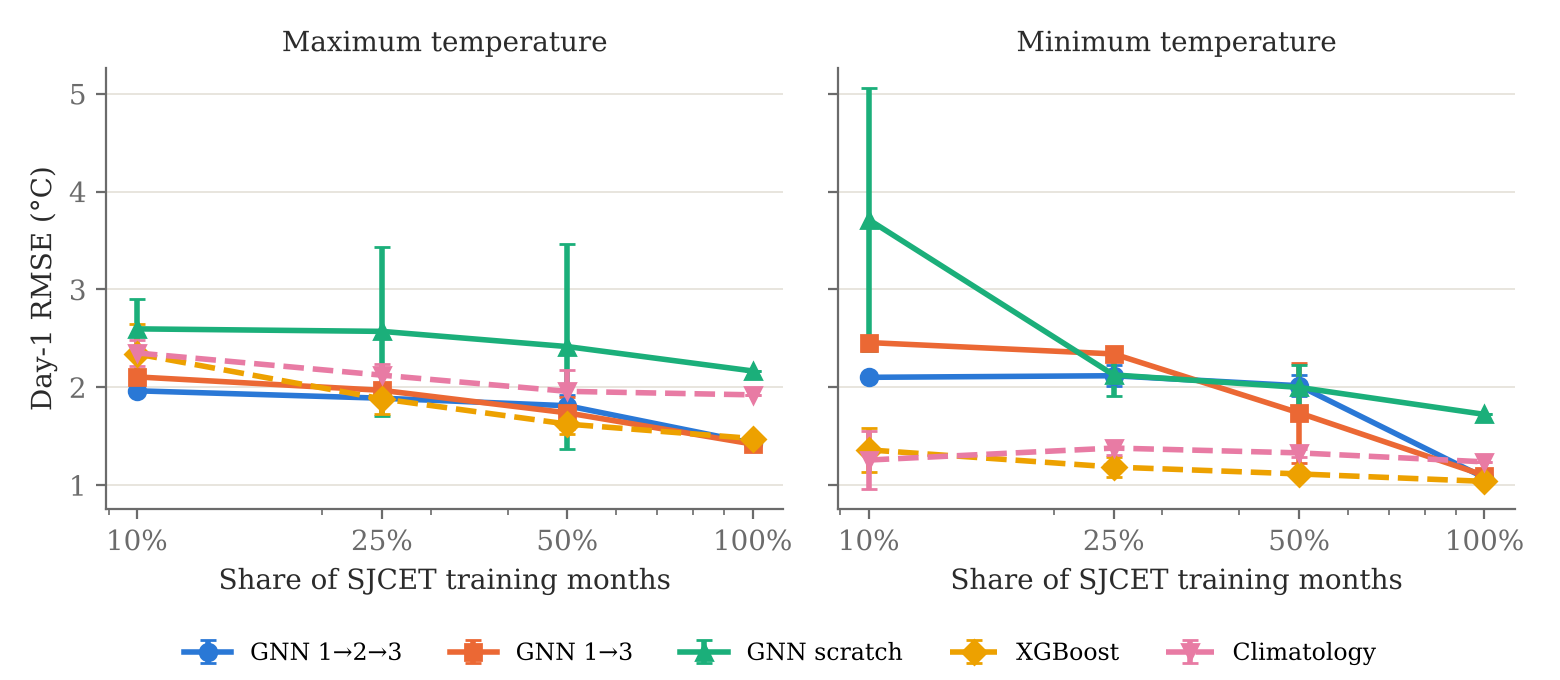
\includegraphics[width=0.98\textwidth]{data_efficiency.png}
    \caption{\capFigEfficiency}\label{fig:efficiency}
\end{figure}

\begin{table}[!htbp]
    \centering
    \caption{\capTabAblation}\label{tab:ablation}
    \footnotesize
    \begin{tabularx}{\textwidth}{|L{3.6cm}|C{1.35cm}|C{1.35cm}|C{1.35cm}|C{1.35cm}|Y|}
        \hline
        \textbf{Model} & \textbf{10\%} & \textbf{25\%} & \textbf{50\%} & \textbf{100\%} & \textbf{Variable} \\ \hline
        GNN 1$\to$\allowbreak{}2$\to$\allowbreak{}3 & \textbf{1.96} & 1.89 & 1.81 & 1.43 & \multirow{5}{*}{Tmax (\textdegree C)} \\ \cline{1-5}
        GNN 1$\to$\allowbreak{}3 & 2.11 & 1.97 & 1.74 & \textbf{1.42} & \\ \cline{1-5}
        GNN from scratch & 2.60 & 2.57 & 2.42 & 2.17 & \\ \cline{1-5}
        XGBoost & 2.34 & \textbf{1.88} & \textbf{1.62} & 1.48 & \\ \cline{1-5}
        Climatology & 2.35 & 2.12 & 1.96 & 1.92 & \\ \hline
        GNN 1$\to$\allowbreak{}2$\to$\allowbreak{}3 & 2.10 & 2.12 & 2.02 & 1.08 & \multirow{5}{*}{Tmin (\textdegree C)} \\ \cline{1-5}
        GNN 1$\to$\allowbreak{}3 & 2.46 & 2.34 & 1.74 & 1.10 & \\ \cline{1-5}
        GNN from scratch & 3.71 & 2.13 & 2.00 & 1.72 & \\ \cline{1-5}
        XGBoost & 1.36 & \textbf{1.18} & \textbf{1.11} & \textbf{1.04} & \\ \cline{1-5}
        Climatology & \textbf{1.26} & 1.38 & 1.33 & 1.24 & \\ \hline
    \end{tabularx}
\end{table}

\begin{itemize}
    \item \textbf{Four months of local data are enough for maximum temperature.} With 10\% of the months, the 1$\to$\allowbreak{}2$\to$\allowbreak{}3 model reaches 1.96\,\textdegree C, the best of all methods, against 2.60\,\textdegree C from scratch.
    \item \textbf{But not for minimum temperature.} With 10--50\% of the months, the pretrained GNNs are worse than climatology and XGBoost for Tmin (2.0--2.5 vs.\ 1.1--1.4\,\textdegree C), because SJCET's minimum varies very little and the network starts from a reanalysis minimum about 1.8\,\textdegree C too warm. This is the clearest negative result of the project.
    \item \textbf{The station stage helps only with little data} (1.96 vs.\ 2.11\,\textdegree C at 10\%); with six stations, none closer than about 50~km, its signal is weak.
\end{itemize}

\section{Live and Seasonal Performance}
\label{sec:res-livelike}

Because the register stops in 2016, a live forecast has no recent SJCET readings. Table~\ref{tab:livelike} scores the models with SJCET's own inputs hidden for the whole test period. The default model loses about 0.5\,\textdegree C on maximum temperature (1.43 to 1.98 at day 1) but hardly anything on minimum temperature (1.08 to 1.17), so the live forecast remains usable, and restoring SJCET's own inputs would recover most of the gap.

\begin{table}[!htbp]
    \centering
    \caption{\capTabLive}\label{tab:livelike}
    \footnotesize
    \begin{tabularx}{\textwidth}{|L{4.2cm}|C{1.7cm}|C{1.7cm}|C{1.7cm}|Y|}
        \hline
        \textbf{Model} & \textbf{Tmax d1} & \textbf{Tmax d6} & \textbf{Tmin d1} & \textbf{Tmin d6} \\ \hline
        GNN 1$\to$\allowbreak{}3 & \textbf{1.80} (1.42) & 1.90 (1.55) & \textbf{1.15} (1.10) & 1.21 (1.25) \\ \hline
        GNN 1$\to$\allowbreak{}2$\to$\allowbreak{}3 & 1.98 (1.43) & 2.05 (1.58) & 1.17 (1.08) & \textbf{1.20} (1.21) \\ \hline
        GNN from scratch & 2.21 (2.17) & \textbf{1.76} (1.85) & 1.63 (1.72) & 1.52 (1.43) \\ \hline
    \end{tabularx}
\end{table}

Table~\ref{tab:season} shows that temperature errors are smallest in the two monsoon seasons, when cloud cover keeps day-to-day changes small, and largest in winter and the pre-monsoon, which is also the season of isolated thunderstorms and the largest rain errors.

\begin{table}[!htbp]
    \centering
    \caption{\capTabSeason}\label{tab:season}
    \footnotesize
    \begin{tabularx}{\textwidth}{|L{4.4cm}|>{\centering\arraybackslash}X|>{\centering\arraybackslash}X|>{\centering\arraybackslash}X|>{\centering\arraybackslash}X|}
        \hline
        \textbf{Model / variable} & \textbf{Winter (Jan--Feb)} & \textbf{Pre-monsoon (Mar--May)} & \textbf{SW monsoon (Jun--Sep)} & \textbf{NE monsoon (Oct--Dec)} \\ \hline
        GNN 1$\to$\allowbreak{}2$\to$\allowbreak{}3, Tmax & 1.85 & 1.52 & 1.24 & 1.22 \\ \hline
        GNN 1$\to$\allowbreak{}2$\to$\allowbreak{}3, Tmin & 1.50 & 1.19 & 0.72 & 0.98 \\ \hline
        GNN 1$\to$\allowbreak{}2$\to$\allowbreak{}3, rain (mm) & 4.1 & 30.3 & 15.6 & 18.8 \\ \hline
        GNN scratch, Tmax & 2.34 & 2.89 & 1.67 & 1.57 \\ \hline
        GNN scratch, Tmin & 1.87 & 2.48 & 0.84 & 1.40 \\ \hline
    \end{tabularx}
\end{table}

\section{Application Interface}
\label{sec:res-app}

The forecasts, the digitized register and the model comparison are presented through a React web application backed by a FastAPI service. The \textbf{Forecast} page shows the live forecast for the coming days and lets a user replay any 2015--2016 date to compare the six-day forecast with what the register recorded, alongside the weather-network map (Figure~\ref{fig:app-forecast}). The \textbf{History} page shows the digitized register as a coverage heat-map, daily readings, and monthly and annual rainfall (Figure~\ref{fig:app-history}). The \textbf{Results} page presents the accuracy and error comparisons of this chapter interactively (Figure~\ref{fig:app-results}).

\begin{figure}[!htbp]
    \centering
    \IfFileExists{figures/app_forecast.png}{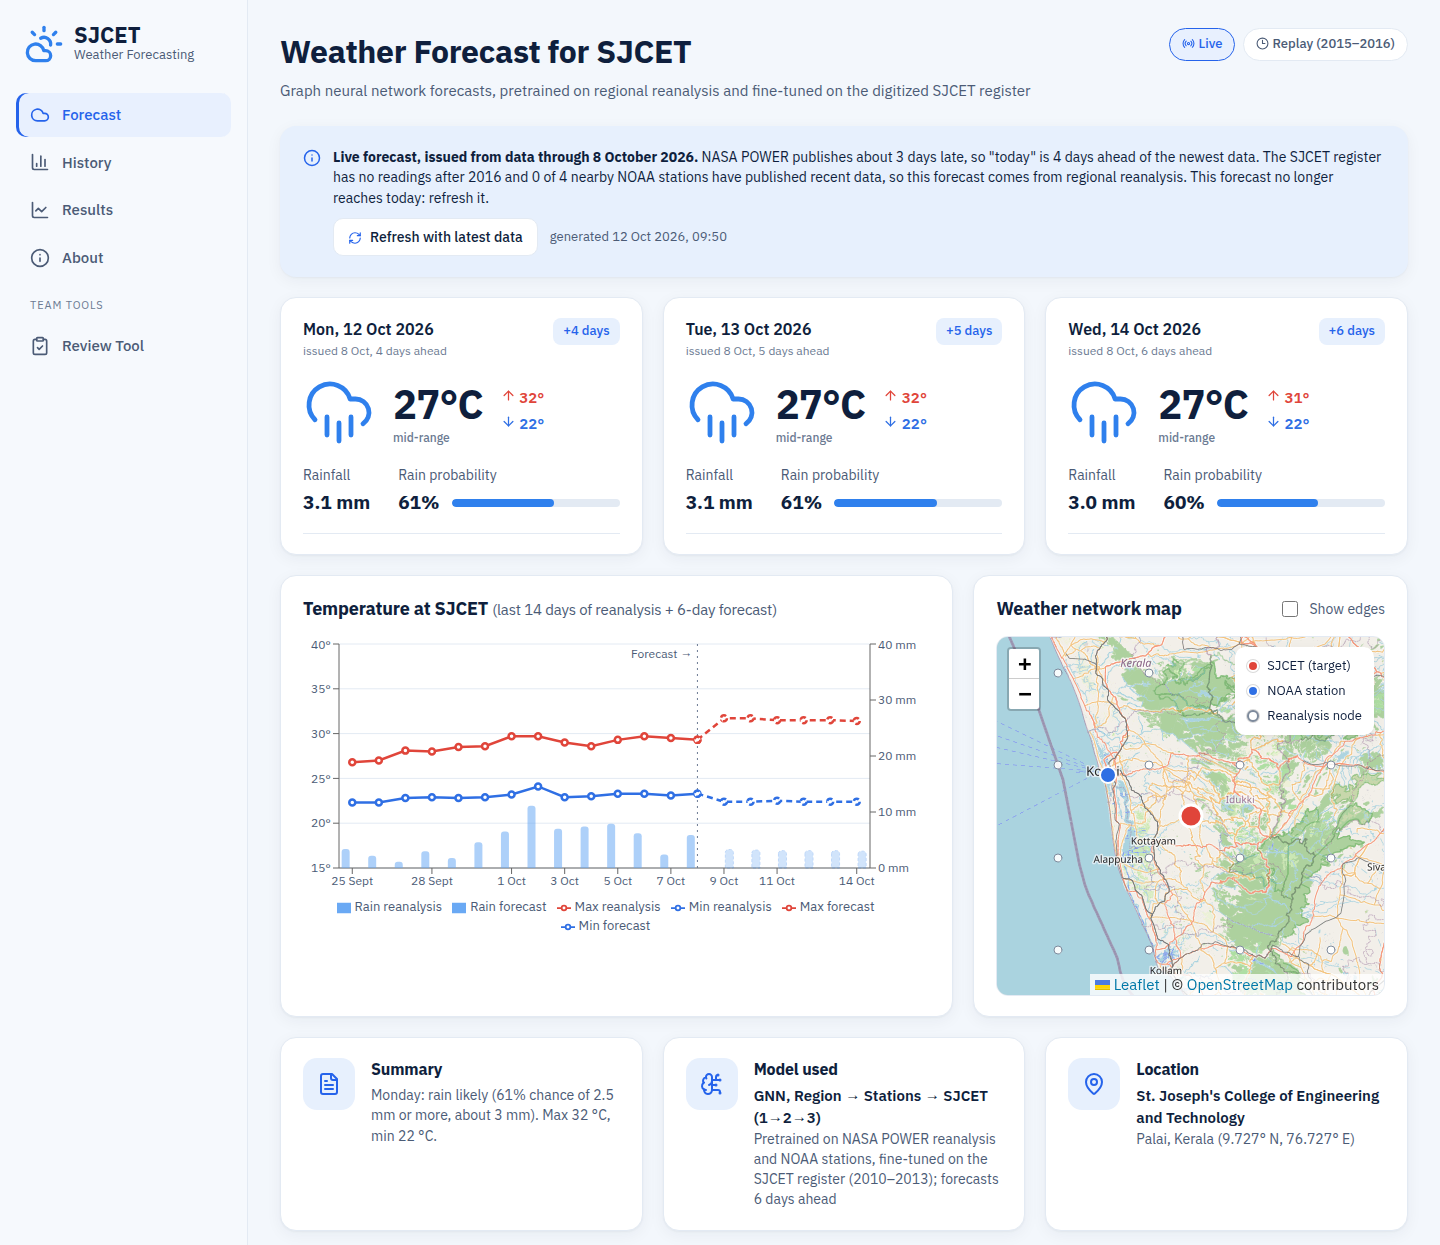
\includegraphics[width=0.9\textwidth]{app_forecast.png}}{\fbox{\parbox[c][5cm][c]{0.85\textwidth}{\centering Screenshot to be added: \textbf{figures/app\_forecast.png}}}}
    \caption{\capFigAppForecast}\label{fig:app-forecast}
\end{figure}

\begin{figure}[!htbp]
    \centering
    \IfFileExists{figures/app_history.png}{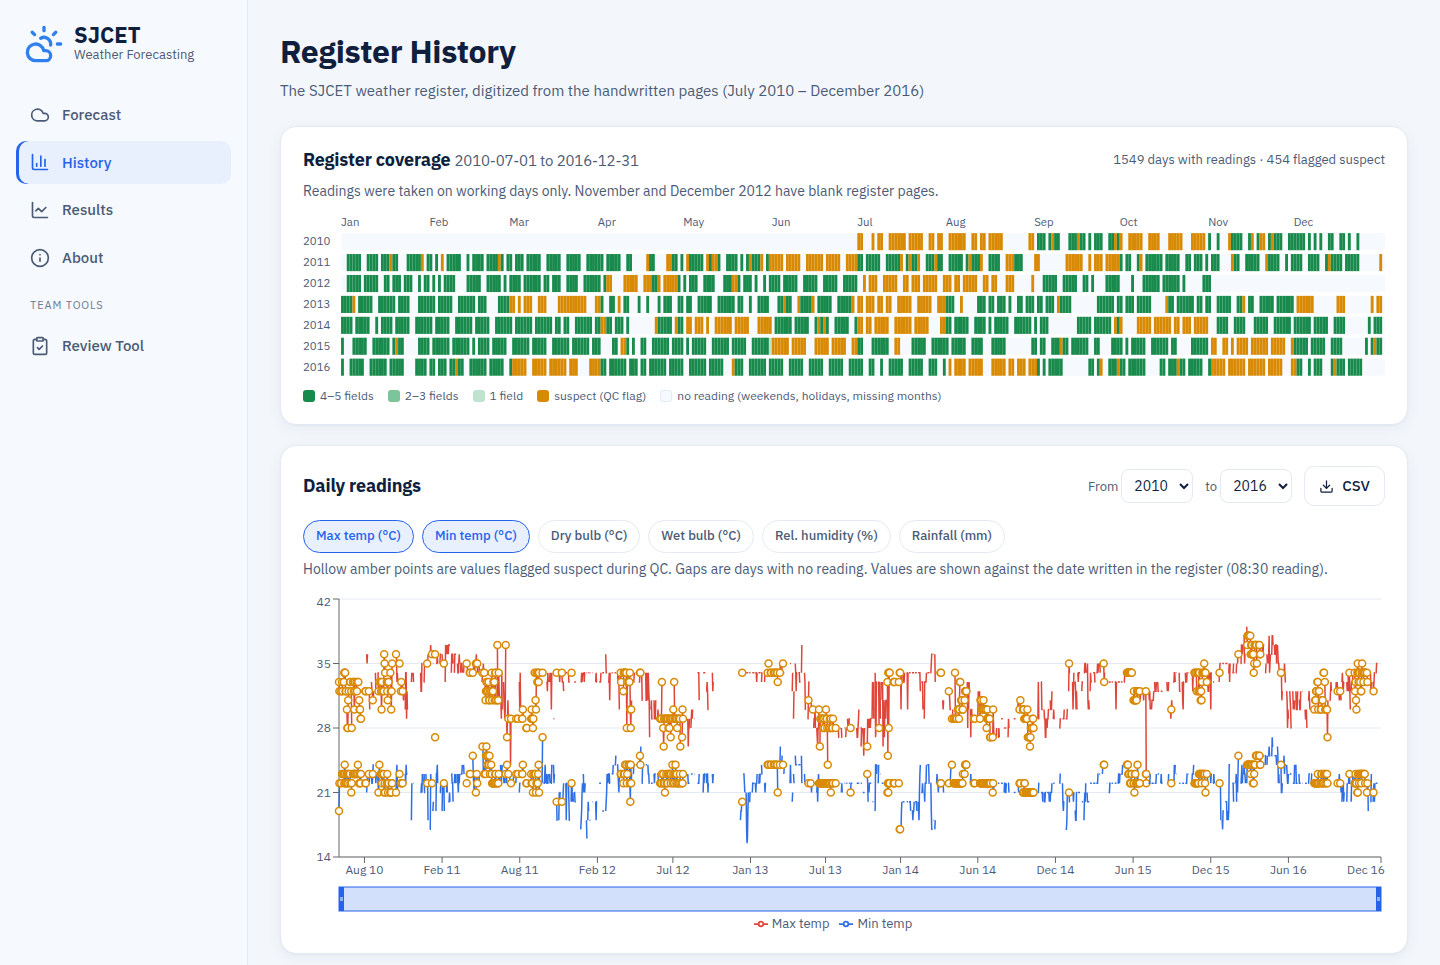
\includegraphics[width=0.9\textwidth]{app_history.png}}{\fbox{\parbox[c][5cm][c]{0.85\textwidth}{\centering Screenshot to be added: \textbf{figures/app\_history.png}}}}
    \caption{\capFigAppHistory}\label{fig:app-history}
\end{figure}

\begin{figure}[!htbp]
    \centering
    \IfFileExists{figures/app_results.png}{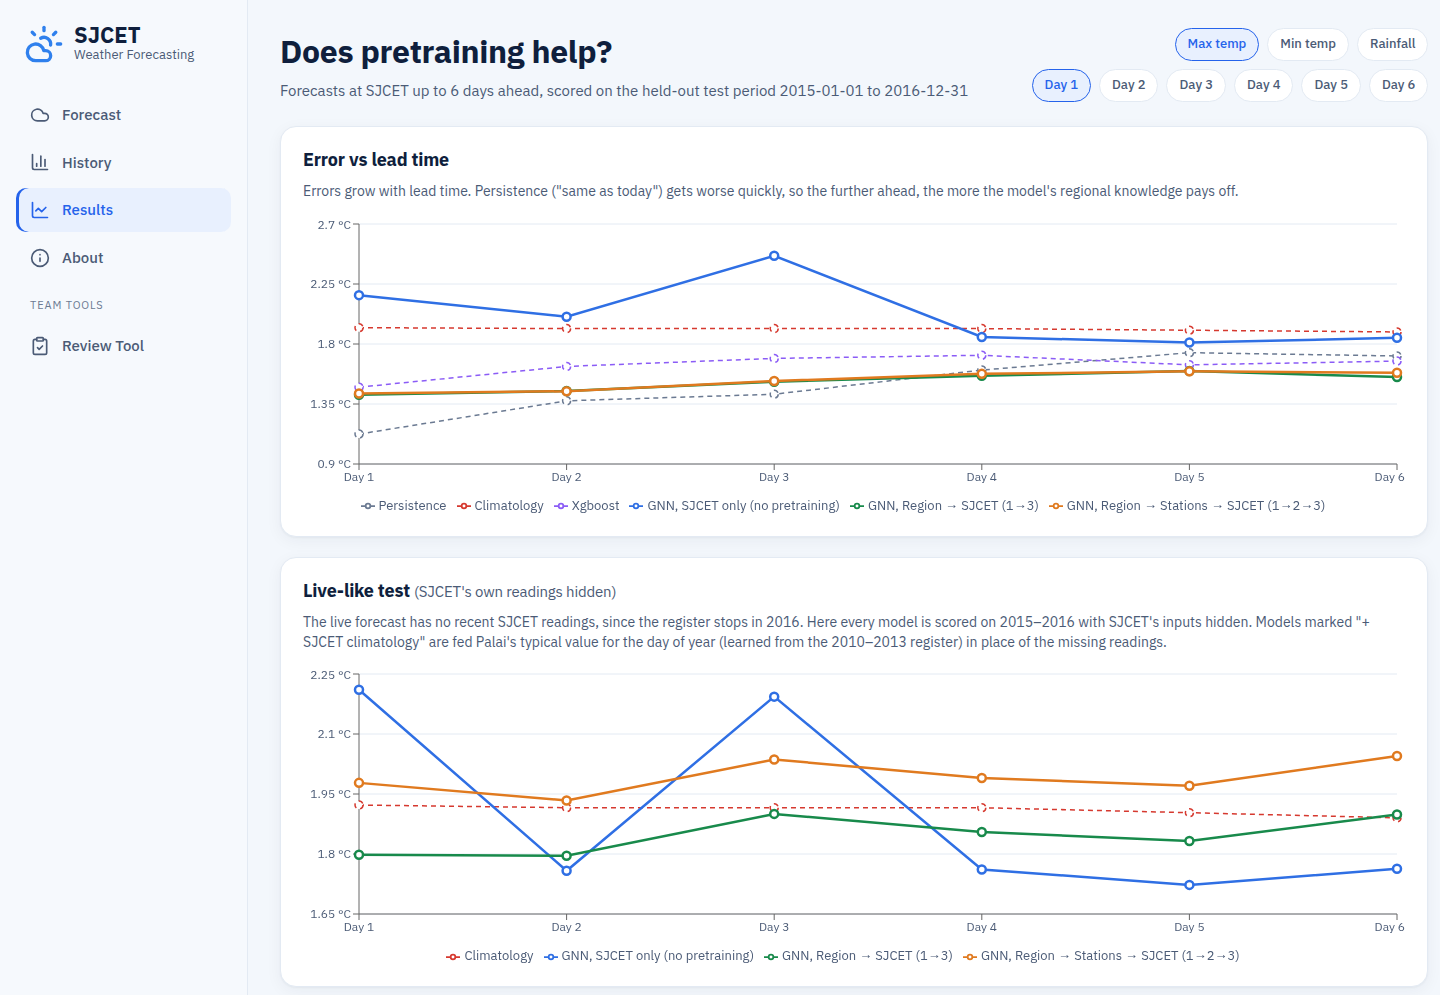
\includegraphics[width=0.9\textwidth]{app_results.png}}{\fbox{\parbox[c][5cm][c]{0.85\textwidth}{\centering Screenshot to be added: \textbf{figures/app\_results.png}}}}
    \caption{\capFigAppResults}\label{fig:app-results}
\end{figure}

\section{Summary of Observations}
\label{sec:res-summary}

\begin{itemize}
    \item The handwritten register was digitized into 1,549 traceable daily records, with 59 of 78 months confirmed against the observers' own totals.
    \item The final model forecasts next-day maximum and minimum temperature with 96.6\% and 96.2\% accuracy, with 86\% and 93\% of forecasts within $\pm$2\,\textdegree C.
    \item Pretraining on regional data lowers the temperature error by about a third and lets the model adapt to SJCET in only two epochs.
    \item With only four months of local data, the pretrained model is the best of all methods for maximum temperature, but worse than climatology for minimum temperature.
    \item The forecast remains usable without SJCET's own recent readings, losing about 0.5\,\textdegree C on maximum temperature.
    \item Rainfall at a single gauge remains the weakest part of the system.
\end{itemize}

\section{Discussion}
\label{sec:discussion}

The Phase 1 results show that staged transfer learning makes a modern forecasting model practical for a station with only a few years of handwritten data. Pretraining on regional reanalysis supplies the weather dynamics, and fine-tuning on the register supplies the local correction from the grid cell to the campus thermometer; together they produce temperature forecasts with about 96\% accuracy. The project's peculiarities shape these results in both directions: the register's whole-degree, often-repeated readings make persistence a hard baseline at one day, and the low variability of the minimum temperature makes climatology hard to beat when local data is scarce.

These conclusions rest on a small test set of a few hundred weekday readings, a reanalysis that carries its own biases, and a single station, so differences of a few hundredths of a degree should not be read as meaningful. In the next phase, the post-2016 photographs will be transcribed to lengthen the record and restore SJCET's inputs to the live forecast, the pretrained model will be combined with the station climatology for low-variance variables, and more and closer reference stations will be added to test the station stage properly.
